
\usetikzlibrary{shadows,arrows}
\usetikzlibrary{decorations.markings}

% Define the layers to draw the diagram
\pgfdeclarelayer{background}
\pgfdeclarelayer{foreground}
\pgfsetlayers{background,main,foreground}



\tikzstyle{packagestyle}=[draw = black!50, fill=orange!15, text width=6.0em, text centered,text = black!70,  minimum height=1.2em]
\tikzstyle{package} = [packagestyle, text width=8em, minimum width=10em, minimum height=1.5em]

% Define block styles  
\tikzstyle{blockstyle}=[draw, fill=blue!20, text width=6.0em, text centered,
  minimum height=1.5em,drop shadow]
\tikzstyle{textbox} = [blockstyle, text width=8em, minimum width=10em,
  minimum height=3em, rounded corners, drop shadow]

\tikzstyle{texto} = [above, text width=6em, text centered]

\tikzset{
    big arrow/.style={
        decoration={markings,mark=at position 1 with {\arrow[scale=2,#1]{>}}},
        postaction={decorate},
        shorten >=0.4pt}}

\newcommand{\class}[2]{node (p#1) [textbox] {#2}}
\newcommand{\package}[2]{node (p#1) [package] {#2}}

\newcommand{\packageback}[4]{%
  \begin{pgfonlayer}{background}
    % Left-top corner of the background rectangle
    \path (#1.west |- #2.north)+(-0.5,0.5) node (a1) {};
    % Right-bottom corner of the background rectanle
    \path (#3.east |- #4.south)+(+0.5,-0.5) node (a2) {};
    % Draw the background
    \path[fill=orange!15,draw=black!50]
      (a1) rectangle (a2);
    % \path (a1.east |- a1.south)+(0.8,-0.3) node (u1)[texto]
      % {\scriptsize\textit{#5}};
    \path (a1.north) + (2.5, 0.2) \package{6} {Backend};
  \end{pgfonlayer}}

\tikzstyle{line} = [draw, thick, color=black!50, big arrow]
% Define distances for bordering

 
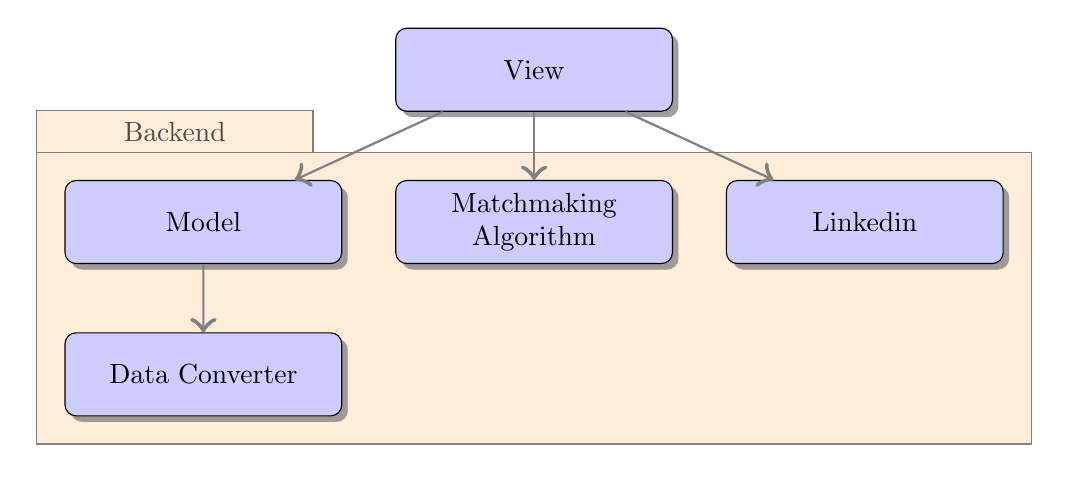
\begin{tikzpicture}[scale = 0.7]
% Draw diagram elements
\path                          \class{1}{View};
\path (p1.south) + ( 0.0, -2.0) \class{2}{Matchmaking Algorithm};
\path (p1.south) + ( 6.0, -2.0) \class{3}{Linkedin};
\path (p1.south) + (-6.0, -2.0) \class{4}{Model};
\path (p4.south) + ( 0.0, -2.0) \class{5}{Data Converter};

% \path (p4.north) + (-0.5, 0.85) \package{6}{Backend};


% Draw arrows between elements
\path [line] (p1) -- node [left] {} (p2);
\path [line] (p1) -- node [left] {} (p3);
\path [line] (p1) -- node [left] {} (p4);
\path [line] (p4) -- node [left] {} (p5);

\packageback{p4}{p4}{p3}{p5}
 
\end{tikzpicture}


